\begin{frame}
\frametitle{Renderizzare Un Triangolo: Demo}
\begin{figure}[ht]
    \centering
    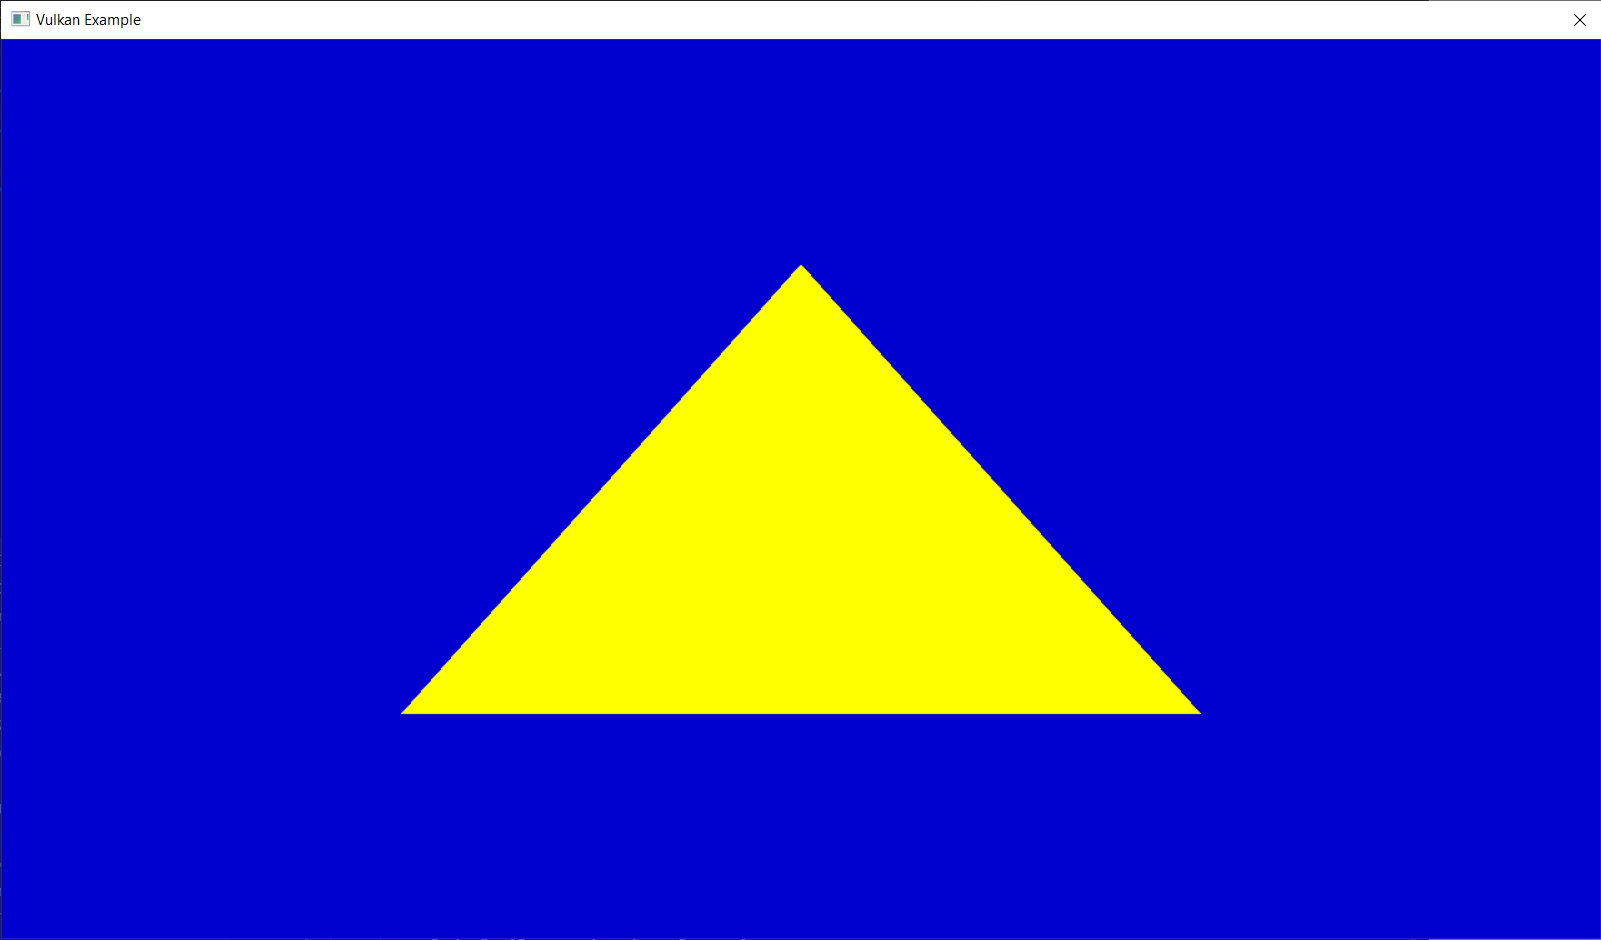
\includegraphics[scale=0.25]{images/SlidesTriangle/Triangle.png}
\end{figure}
\end{frame}

\begin{frame}
\frametitle{Renderizzare Un Triangolo: Vertex Shader}
\lstinputlisting[language=C++]{src/SlidesTriangle/shader.vert}
\end{frame}

\begin{frame}
\frametitle{Renderizzare Un Triangolo: Fragment Shader}
\lstinputlisting[language=C++]{src/SlidesTriangle/shader.frag}
\end{frame}

\begin{frame}
\frametitle{Renderizzare Un Triangolo}
\begin{itemize}
\item Usiamo un pipeline state object per descrivere l'intero stato della pipeline grafica
\item Un pipeline state object descrive anche quali shader utilizzare
\item Sul command buffer, scriviamo un comando che indica alla GPU di configurare lo stato della pipeline grafica usando il pipeline state object da noi creato
\item Sempre sul command buffer, scriviamo un comando che attiva la pipeline grafica per renderizzare tre vertici
\end{itemize}
\end{frame}
